\documentclass[a4paper]{article} 

\title{\textcolor{blue}{Sunset Crater Rock Lichen Analyses}}  
\author{Matthew K. Lau}

%Sweave package
\usepackage{/Library/Frameworks/R.framework/Resources/share/texmf/Sweave}
\usepackage[utf8x]{inputenc} %this is to fix the quote corruption post sweaving

%Miscellaneaous
\usepackage[margin=2cm]{geometry}
\usepackage{color}
\usepackage{hyperref}
\hypersetup{colorlinks=false}

%packages for the flow diagram
\usepackage{tikz}
\usetikzlibrary{shapes,arrows}

%Tikz styles
% styles for flowcharts
%\tikzstyle{decision} = [diamond, draw, fill=green!15,text width=4.5em, text badly centered, node distance=3cm, inner sep=0pt]
\tikzstyle{block} = [rectangle, draw, fill=white!10, text width=5em, text centered, minimum height=4em]
\tikzstyle{blockr} = [rectangle, draw, fill=white!10, text width=5em, text centered, minimum height=4em,rounded corners]
%\tikzstyle{blockorange} = [rectangle, draw,fill=orange!15, text width=5em, text centered, rounded corners, minimum height=4em]

%Graphics Location
\graphicspath{{images/}}

\begin{document}

\maketitle

\setcounter{tocdepth}{2}
\tableofcontents

\section{Notes on data analyses}
\begin{description}
\item My overall approach here is to analyze what I'm referring to as univariate (i.e., abundance, richness and diversity) and multivariate community statistics.
\item[*] I removed dead trees from the analysis. They did not correlate well with moth susceptibility and unnecessarily complicated analyses.
\item I first proceed through the analyses of the univariate and multivariate statistics using moth susceptibility (variable name = \texttt{Moth}) as a single predictor. This allows us to first see if there is some potential effect of moth susceptibility. Here, I did use the pairing scheme (variable name = \texttt{Tree.pairs}) in the analyses to factor out environmental noise.
\item I then conducted a series of analyses looking at the relationship between moth susceptibility and various factors that had good correlations with the community composition based on vector analysis of the NMS ordination.
\item Next, I used multiple regressions and PerMANOVA to look at the effects of these factors on the univariate and multivariate community response variables.
\item Last, I used SEM (Structural Equation Modeling) to begin to tease apart a mechanistic story of how moth susceptibility affects the rock lichen/moss community. Since tree pairing did not have a statistically significant effect on community composition or show any relationship with any of the other predictor variables, I did not include it in any of the SEMs. This will only make the results conservative, because we are not using it to account for environmental variation.
\end{description}

%%Import Data

\begin{Schunk}
\begin{Sinput}
> summary(com)
\end{Sinput}
\begin{Soutput}
     Acacon            Acasup         Acaobp         Sterile.sp   
 Min.   :0.00000   Min.   :0.00   Min.   :0.0000   Min.   :0.000  
 1st Qu.:0.00000   1st Qu.:0.00   1st Qu.:0.0000   1st Qu.:0.000  
 Median :0.00000   Median :0.05   Median :0.0000   Median :0.000  
 Mean   :0.02833   Mean   :0.14   Mean   :0.1493   Mean   :0.001  
 3rd Qu.:0.02500   3rd Qu.:0.17   3rd Qu.:0.0200   3rd Qu.:0.000  
 Max.   :0.26000   Max.   :1.04   Max.   :8.0000   Max.   :0.060  
    Brown.cr     Lobalp             Canros           Calare       
 Min.   :0   Min.   :0.000000   Min.   :0.0000   Min.   :0.00000  
 1st Qu.:0   1st Qu.:0.000000   1st Qu.:0.0000   1st Qu.:0.00000  
 Median :0   Median :0.000000   Median :0.1400   Median :0.00000  
 Mean   :0   Mean   :0.002333   Mean   :0.3202   Mean   :0.01967  
 3rd Qu.:0   3rd Qu.:0.000000   3rd Qu.:0.4225   3rd Qu.:0.00000  
 Max.   :0   Max.   :0.040000   Max.   :1.7000   Max.   :0.56000  
     Phydub            Rhichr           Xanlin           Xanpli      
 Min.   :0.00000   Min.   :0.0000   Min.   :0.0000   Min.   :0.0000  
 1st Qu.:0.00000   1st Qu.:0.0000   1st Qu.:0.0000   1st Qu.:0.0000  
 Median :0.00000   Median :0.0400   Median :0.0300   Median :0.0000  
 Mean   :0.09633   Mean   :0.2915   Mean   :0.6223   Mean   :0.2115  
 3rd Qu.:0.09500   3rd Qu.:0.3650   3rd Qu.:0.7025   3rd Qu.:0.2450  
 Max.   :1.19000   Max.   :2.8500   Max.   :5.9300   Max.   :1.6300  
     Xanele           GrBr.cr             Gray.cr      
 Min.   :0.00000   Min.   :0.0000000   Min.   :0.0000  
 1st Qu.:0.00000   1st Qu.:0.0000000   1st Qu.:0.0000  
 Median :0.00000   Median :0.0000000   Median :0.0000  
 Mean   :0.03867   Mean   :0.0006667   Mean   :0.0025  
 3rd Qu.:0.00000   3rd Qu.:0.0000000   3rd Qu.:0.0000  
 Max.   :0.81000   Max.   :0.0400000   Max.   :0.0700  
     Synrur        Cerpur.Bryarg     
 Min.   :0.00000   Min.   :0.000000  
 1st Qu.:0.00000   1st Qu.:0.000000  
 Median :0.00000   Median :0.000000  
 Mean   :0.04933   Mean   :0.008667  
 3rd Qu.:0.00000   3rd Qu.:0.000000  
 Max.   :1.70000   Max.   :0.410000  
\end{Soutput}
\begin{Sinput}
> summary(env)
\end{Sinput}
\begin{Soutput}
   Tree.pairs        Moth        Litter..       Big.rocks..    
 Min.   : 1.0   Min.   :0.0   Min.   : 19.04   Min.   : 0.000  
 1st Qu.: 8.0   1st Qu.:0.0   1st Qu.: 73.89   1st Qu.: 2.322  
 Median :15.5   Median :0.5   Median : 86.39   Median :11.575  
 Mean   :15.5   Mean   :0.5   Mean   : 79.81   Mean   :14.901  
 3rd Qu.:23.0   3rd Qu.:1.0   3rd Qu.: 95.82   3rd Qu.:19.995  
 Max.   :30.0   Max.   :1.0   Max.   :100.00   Max.   :59.670  
 Small.rocks..       Shrubs..         Grass..          Branches..   
 Min.   : 0.000   Min.   :0.0000   Min.   :0.00000   Min.   :0.000  
 1st Qu.: 0.000   1st Qu.:0.0000   1st Qu.:0.00000   1st Qu.:0.000  
 Median : 0.000   Median :0.0000   Median :0.00000   Median :0.000  
 Mean   : 4.798   Mean   :0.4057   Mean   :0.02467   Mean   :0.071  
 3rd Qu.: 3.072   3rd Qu.:0.0000   3rd Qu.:0.00000   3rd Qu.:0.000  
 Max.   :35.370   Max.   :7.5900   Max.   :1.48000   Max.   :4.260  
   Light...N       Light...S     Light...average 
 Min.   : 1.80   Min.   : 1.80   Min.   : 2.400  
 1st Qu.: 8.00   1st Qu.: 9.70   1st Qu.: 9.213  
 Median :15.00   Median :16.00   Median :16.050  
 Mean   :17.68   Mean   :17.81   Mean   :17.743  
 3rd Qu.:26.10   3rd Qu.:26.15   3rd Qu.:25.525  
 Max.   :45.10   Max.   :44.60   Max.   :41.300  
\end{Soutput}
\end{Schunk}

\begin{Schunk}
\begin{Sinput}
> library(vegan)
> library(gplots)
> attach(env)
\end{Sinput}
\end{Schunk}

\section{Species Accumulation Curves}

Although the sampling curves are not fully asymptotic, they are beginning to level off, which to me suggests that sampling is at an acceptable level.

\begin{Schunk}
\begin{Sinput}
> par(mfrow = c(1, 2))
> plot(specaccum(com), lwd = 0.5, xlab = "Trees Sampled", 
+     ylab = "Species Number", main = "All Trees")
> plot(specaccum(com[tree == 1, ]), add = FALSE, xlab = "Trees Sampled", 
+     ylab = "Species Number")
> abline(h = 15, lwd = 0.3, lty = 2)
> plot(specaccum(com[tree == 0, ]), add = TRUE, col = "red")
> abline(h = 13, lwd = 0.3, lty = 2)
> legend("bottomright", c("S", "R"), lty = 1, col = c("black", 
+     "red"), bty = "n")
\end{Sinput}
\end{Schunk}
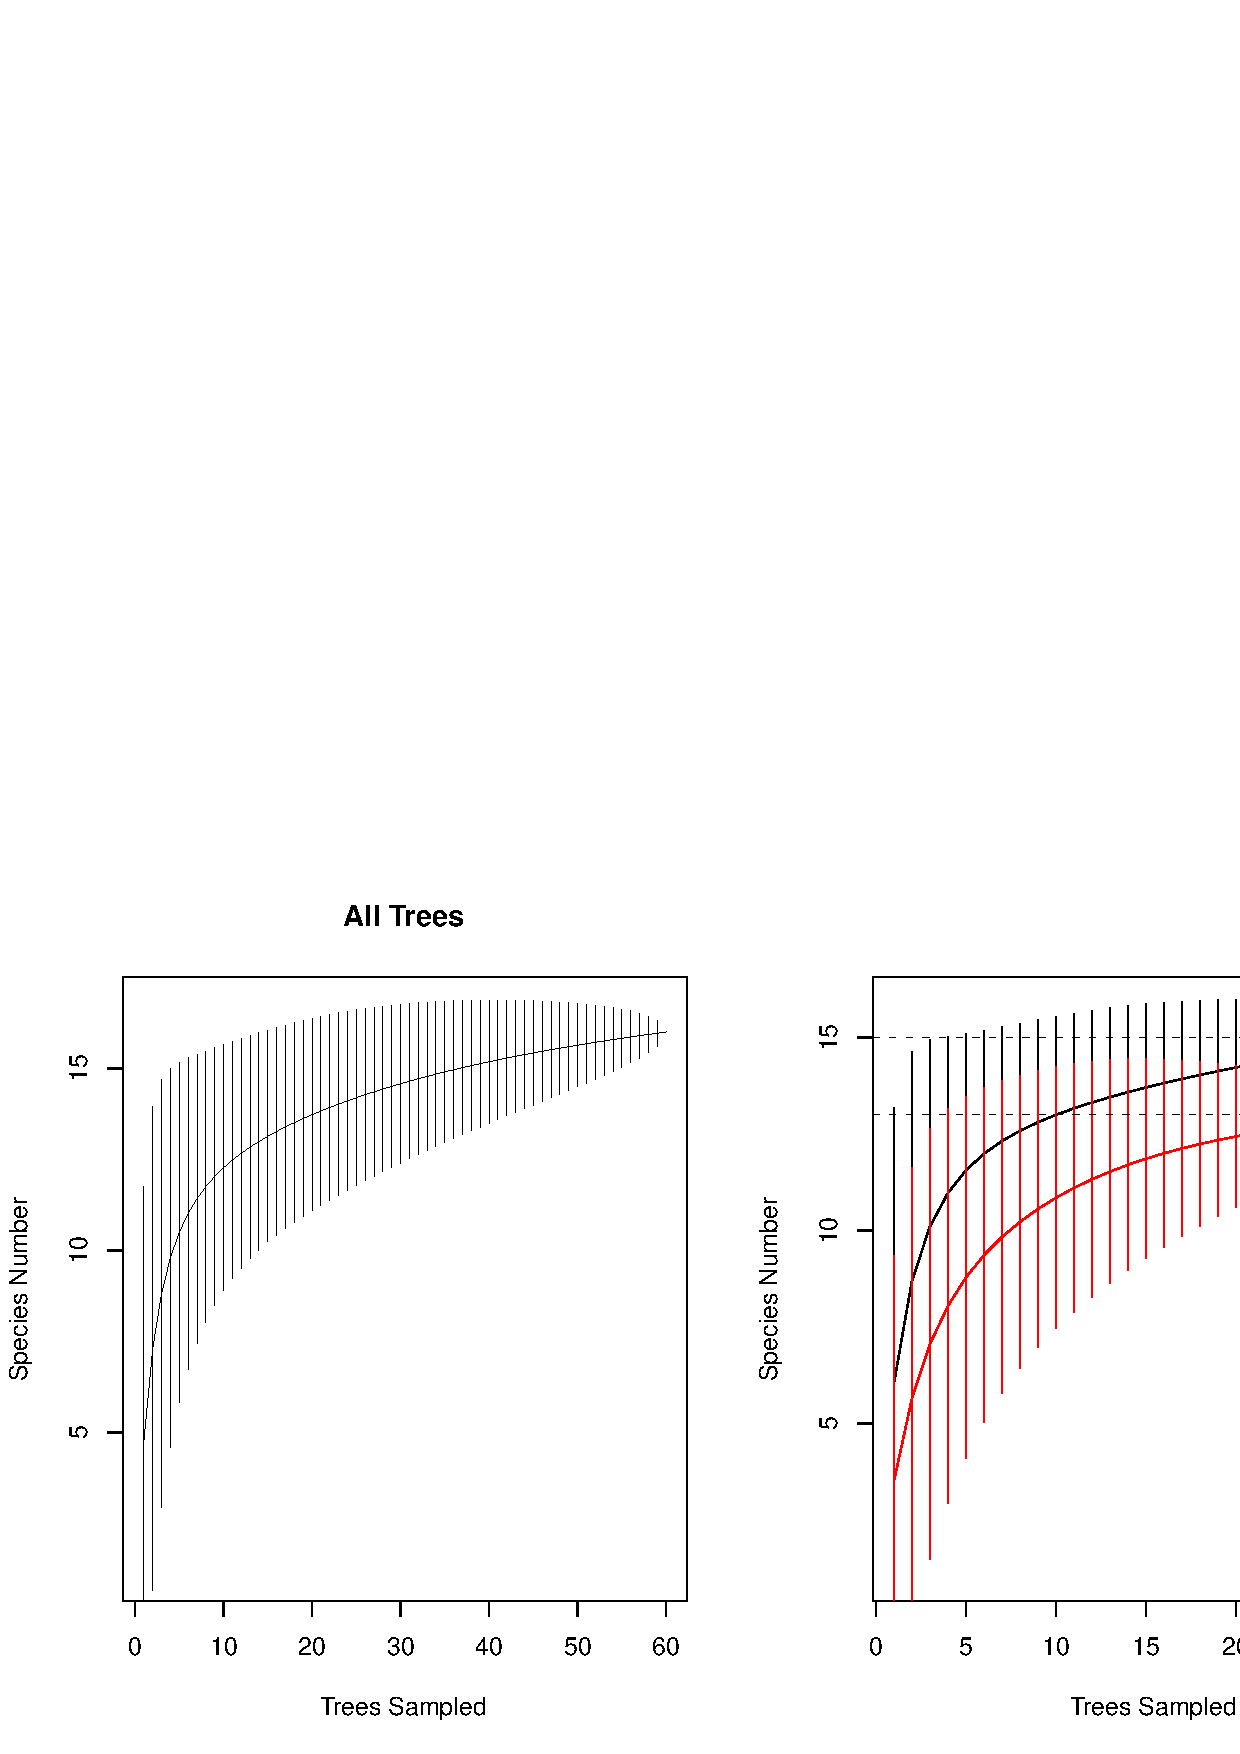
\includegraphics{SCRL_tex-004}


\section{Univariate Community Analyses}

All of the univariate summary statistics (abundance, species richness and Shannon's diversity index) were significantly increased by moth resistance.

\subsection{Abundance}

\begin{Schunk}
\begin{Sinput}
> a = apply(com, 1, sum)
> wilcox.test(a, y = Tree.pairs, alternative = "less", 
+     paired = TRUE)
\end{Sinput}
\begin{Soutput}
	Wilcoxon signed rank test with continuity correction

data:  a and Tree.pairs 
V = 47, p-value = 8.501e-11
alternative hypothesis: true location shift is less than 0 
\end{Soutput}
\end{Schunk}

\subsection{Species Richness}

\begin{Schunk}
\begin{Sinput}
> r = com
> r[r != 0] <- 1
> r = apply(r, 1, sum)
> wilcox.test(r, y = Tree.pairs, alternative = "less", 
+     paired = TRUE)
\end{Sinput}
\begin{Soutput}
	Wilcoxon signed rank test with continuity correction

data:  r and Tree.pairs 
V = 107.5, p-value = 8.975e-09
alternative hypothesis: true location shift is less than 0 
\end{Soutput}
\end{Schunk}

\subsection{Shannon's Diversity Index}

\begin{Schunk}
\begin{Sinput}
> h = diversity(com)
> wilcox.test(h, y = Tree.pairs, alternative = "less", 
+     paired = TRUE)
\end{Sinput}
\begin{Soutput}
	Wilcoxon signed rank test with continuity correction

data:  h and Tree.pairs 
V = 5, p-value = 1.075e-11
alternative hypothesis: true location shift is less than 0 
\end{Soutput}
\end{Schunk}

\subsection{Barplot of Abundance, Richness and Diversity Response to Moth Resistance}

\begin{Schunk}
\begin{Sinput}
> se = function(x) {
+     sd(x)/sqrt(length(x))
+ }
> par(mfrow = c(1, 3))
> barplot2(tapply(a, tree, mean), xlab = "Resistance", 
+     ylab = "Percent Abundance", plot.ci = TRUE, ci.u = tapply(a, 
+         tree, mean) + tapply(a, tree, se), ci.l = tapply(a, 
+         tree, mean) - tapply(a, tree, se))
> barplot2(tapply(r, tree, mean), xlab = "Resistance", 
+     ylab = "Species Richness", plot.ci = TRUE, ci.u = tapply(r, 
+         tree, mean) + tapply(r, tree, se), ci.l = tapply(r, 
+         tree, mean) - tapply(r, tree, se))
> barplot2(tapply(h, tree, mean), xlab = "Resistance", 
+     ylab = "Shannon Index", plot.ci = TRUE, ci.u = tapply(h, 
+         tree, mean) + tapply(h, tree, se), ci.l = tapply(h, 
+         tree, mean) - tapply(h, tree, se))
\end{Sinput}
\end{Schunk}
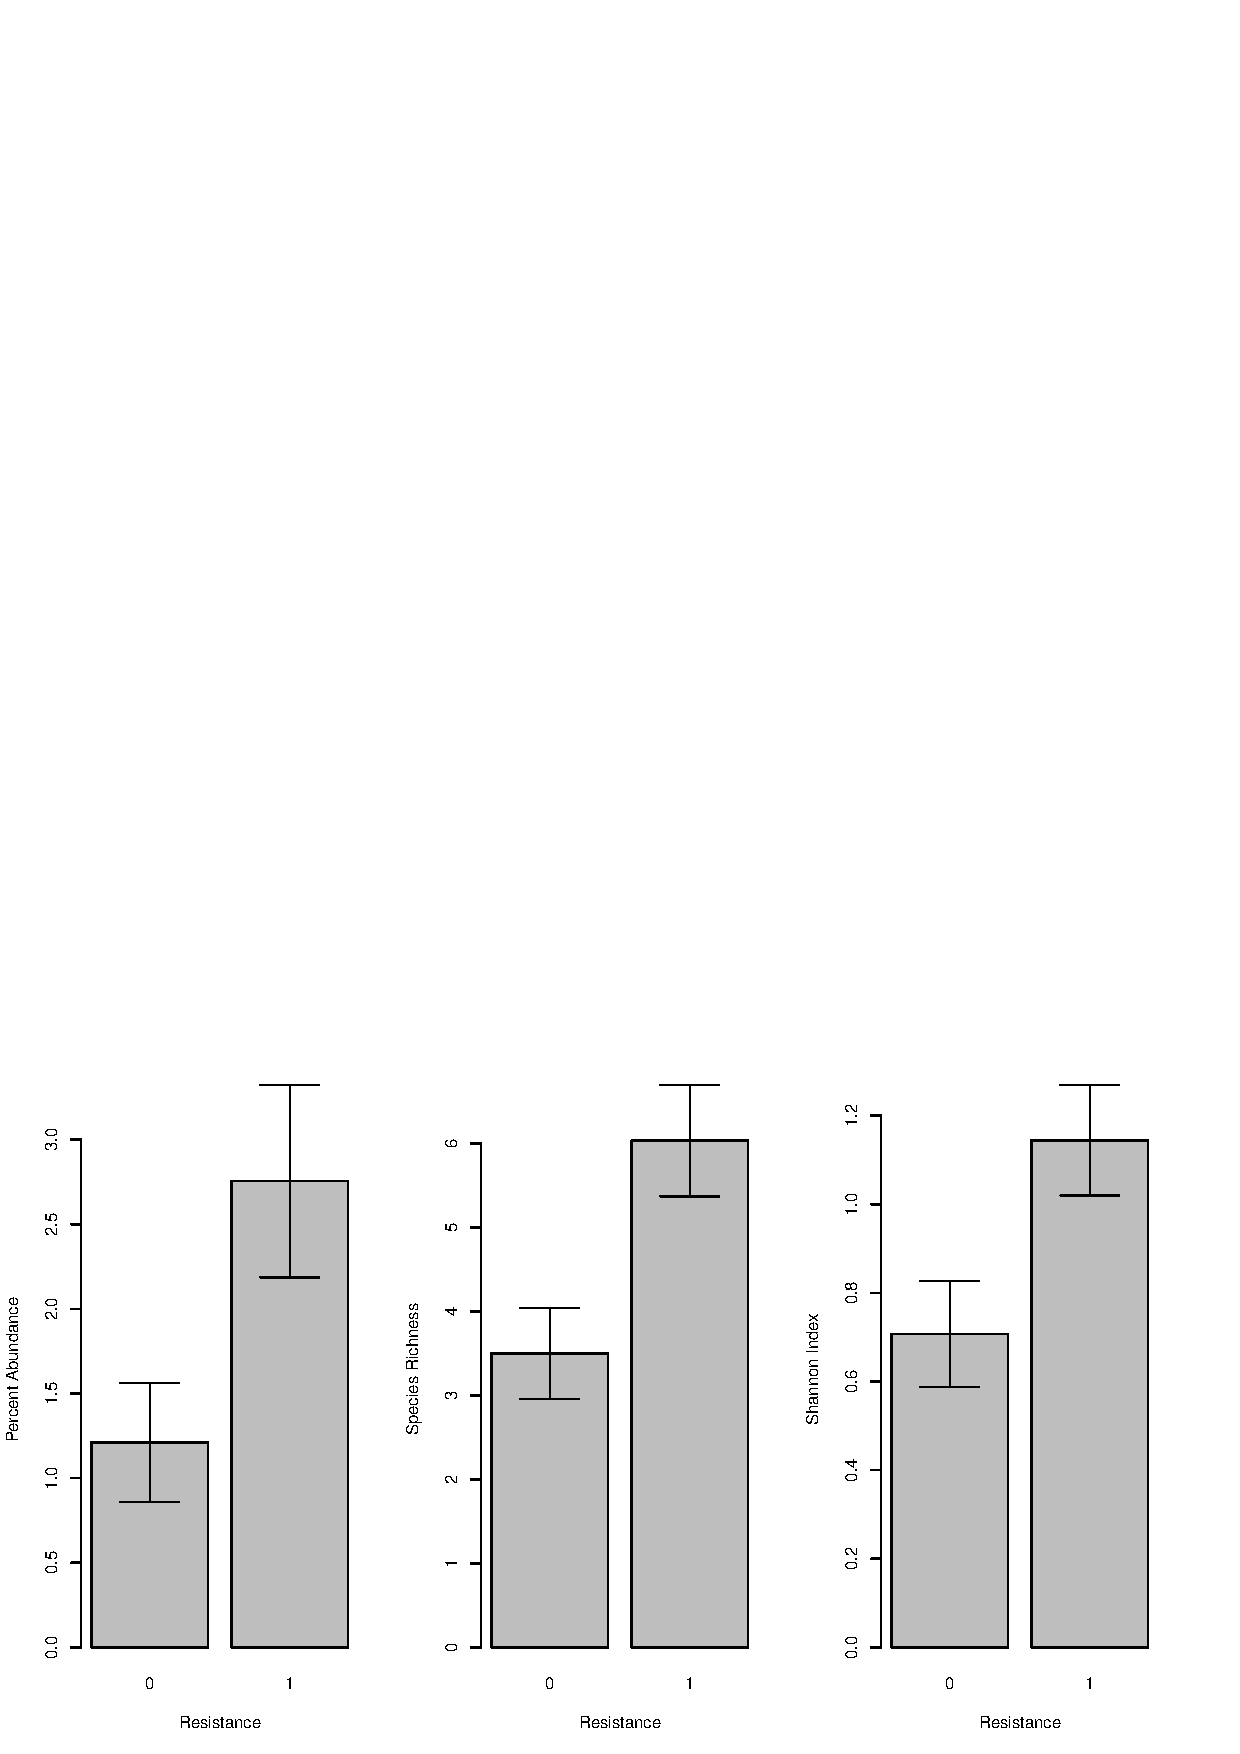
\includegraphics{SCRL_tex-008}

\section{Multivariate Community Analyses}

\subsection{Pairwise Plot of Species with at Least 5\% Total Abundance}

\begin{Schunk}
\begin{Sinput}
> source("/Users/artemis/Documents/R_Docs/Scripts/Functions/pairs.R")
> pairs(com[apply(com, 2, sum) >= 5], lower.panel = panel.cor, 
+     upper.panel = panel.lmr)
\end{Sinput}
\end{Schunk}
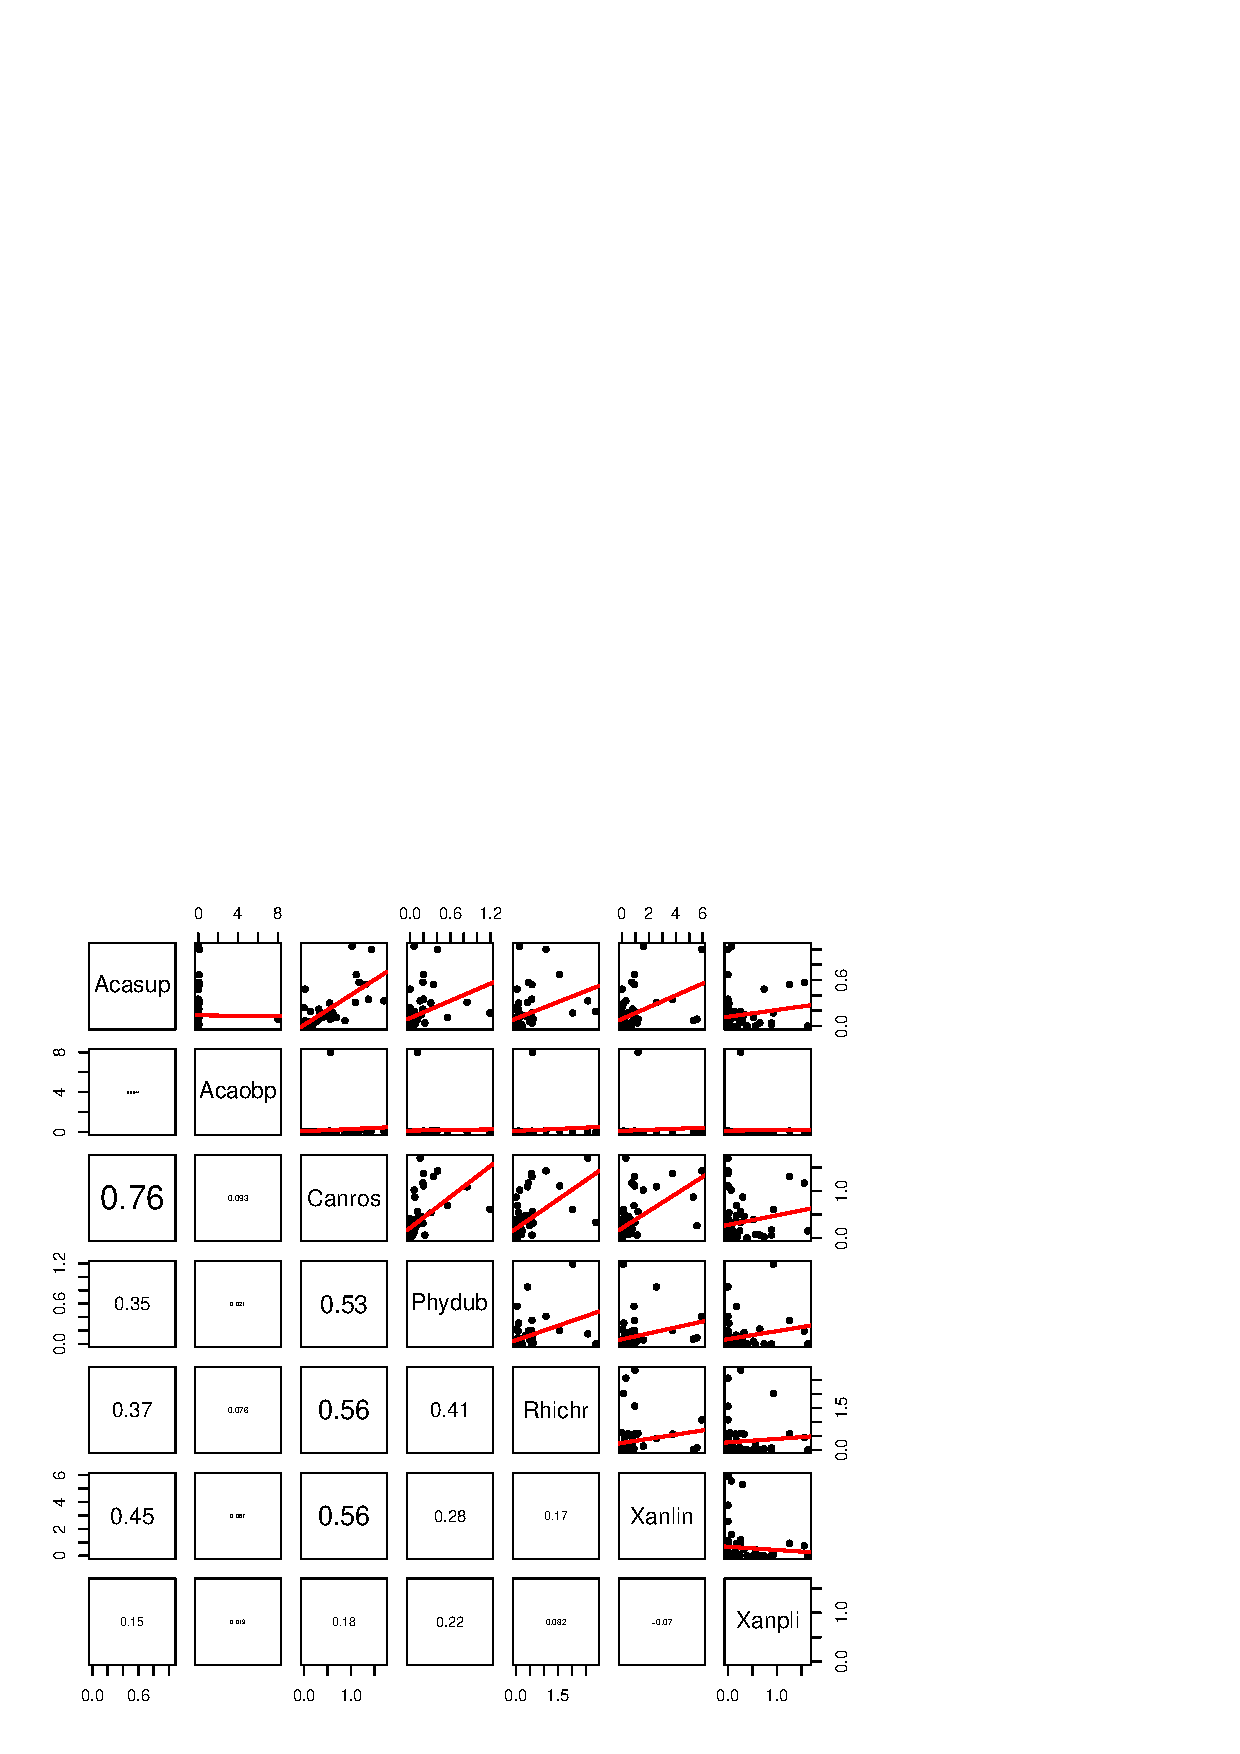
\includegraphics{SCRL_tex-009}

\subsection{PerMANOVA}

\begin{Schunk}
\begin{Sinput}
> d = vegdist(cbind(com, rep(0.01, nrow(com))))
> adonis(d ~ Moth + Tree.pairs/Moth, permutations = 99999)
\end{Sinput}
\begin{Soutput}
Call:
adonis(formula = d ~ Moth + Tree.pairs/Moth, permutations = 99999) 

                      Df SumsOfSqs  MeanSqs  F.Model     R2  Pr(>F)  
Moth             1.00000   0.88978  0.88978  2.81680 0.0441 0.01682 *
Tree.pairs       1.00000   0.65644  0.65644  2.07814 0.0326 0.05763 .
Moth:Tree.pairs  1.00000   0.92389  0.92389  2.92479 0.0458 0.01391 *
Residuals       56.00000  17.68936  0.31588          0.8775          
Total           59.00000  20.15947                   1.0000          
---
Signif. codes:  0 ‘***’ 0.001 ‘**’ 0.01 ‘*’ 0.05 ‘.’ 0.1 ‘ ’ 1 
\end{Soutput}
\end{Schunk}

\subsection{Indicator Species Analysis}

\begin{Schunk}
\begin{Sinput}
> library(labdsv)
> indsp = indval(com, (tree + 1))
> summary(indsp)
\end{Sinput}
\begin{Soutput}
       cluster indicator_value probability
Canros       2          0.6397       0.002
Acasup       2          0.6295       0.002
Acacon       2          0.4769       0.001
Acaobp       2          0.4241       0.010
Phydub       2          0.4125       0.025
Calare       2          0.2966       0.034

Sum of probabilities                 =  6.669 

Sum of Indicator Values              =  4.64 

Sum of Significant Indicator Values  =  2.88 

Number of Significant Indicators     =  6 

Significant Indicator Distribution

2 
6 
\end{Soutput}
\begin{Sinput}
> detach(package:labdsv)
\end{Sinput}
\end{Schunk}

\subsection{Ordination with Vectors}

\begin{Schunk}
\begin{Sinput}
> nms.x = read.csv("moth_nms.csv")
> plot(nms.x, col = (env$Moth + 1))
> fit = envfit(nms.x, env[, c(-9, -10)], permutations = 99999)
> plot(fit, col = "black")
\end{Sinput}
\end{Schunk}
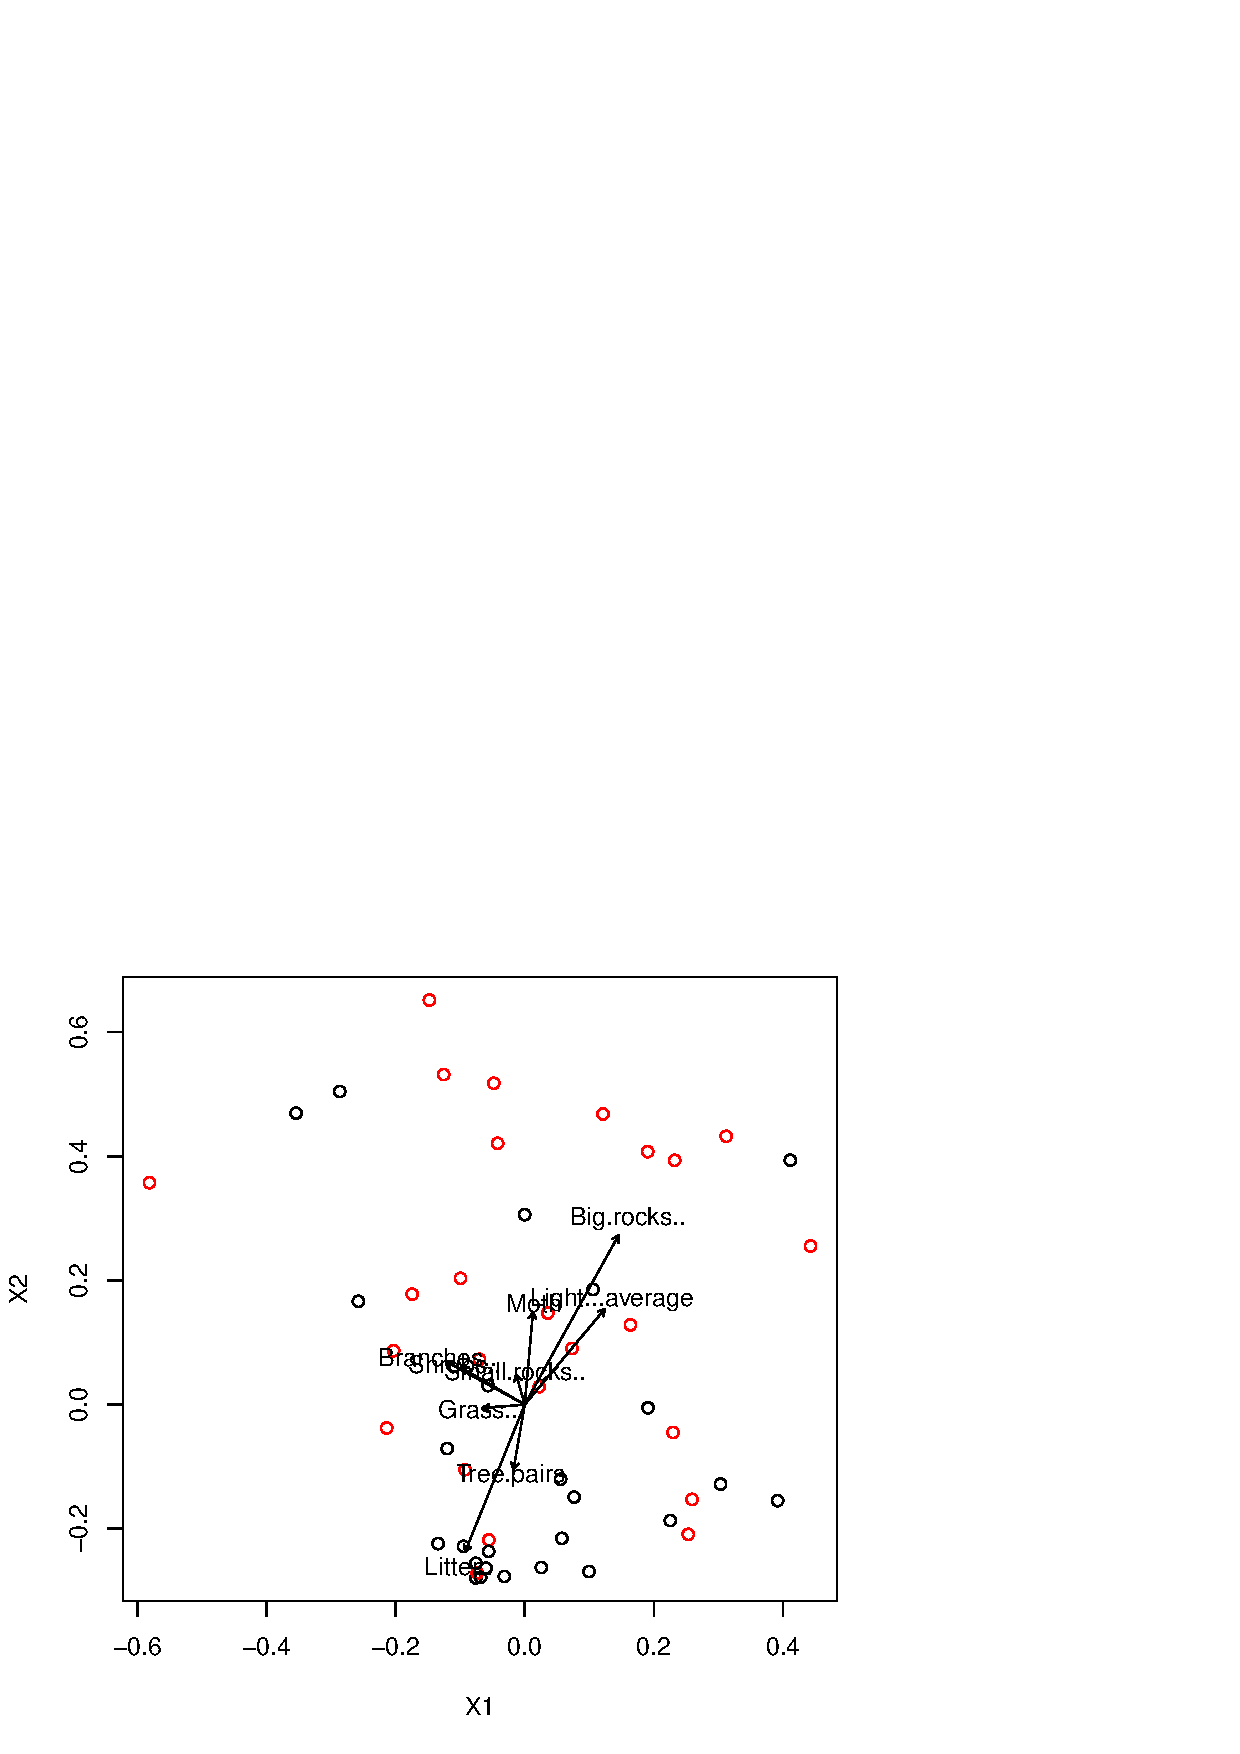
\includegraphics{SCRL_tex-012}

\subsubsection{Analysis of NMS Ordination Vector}
\begin{Schunk}
\begin{Sinput}
> fit
\end{Sinput}
\begin{Soutput}
***VECTORS

                       X1        X2     r2  Pr(>r)    
Tree.pairs      -0.163158 -0.986600 0.0605 0.16812    
Moth             0.085751  0.996317 0.1206 0.02574 *  
Litter..        -0.362543 -0.931967 0.3502   3e-05 ***
Big.rocks..      0.470257  0.882530 0.5148   1e-05 ***
Small.rocks..   -0.264370  0.964421 0.0138 0.67347    
Shrubs..        -0.855552  0.517717 0.0719 0.11165    
Grass..         -0.996016 -0.089179 0.0229 0.33554    
Branches..      -0.869419  0.494076 0.1061 0.04987 *  
Light...average  0.627335  0.778749 0.2112 0.00121 ** 
---
Signif. codes:  0 ‘***’ 0.001 ‘**’ 0.01 ‘*’ 0.05 ‘.’ 0.1 ‘ ’ 1 
P values based on 99999 permutations.
\end{Soutput}
\end{Schunk}

\section{Mechanistic Explorations of the Effects of Moth Resistance}

\subsection{Relationship between Moth Resistance and Factors}

\begin{Schunk}
\begin{Sinput}
> pairs(cbind(Moth, Litter.., Big.rocks.., Small.rocks.., 
+     Light...average), lower.panel = panel.cor, upper.panel = panel.lmr)
> cor.test(Litter.., Moth)
\end{Sinput}
\begin{Soutput}
	Pearson's product-moment correlation

data:  Litter.. and Moth 
t = -3.0871, df = 58, p-value = 0.003098
alternative hypothesis: true correlation is not equal to 0 
95 percent confidence interval:
 -0.5747658 -0.1345822 
sample estimates:
       cor 
-0.3756689 
\end{Soutput}
\begin{Sinput}
> cor.test(Big.rocks.., Moth)
\end{Sinput}
\begin{Soutput}
	Pearson's product-moment correlation

data:  Big.rocks.. and Moth 
t = 2.6217, df = 58, p-value = 0.01115
alternative hypothesis: true correlation is not equal to 0 
95 percent confidence interval:
 0.07802678 0.53519178 
sample estimates:
      cor 
0.3255023 
\end{Soutput}
\begin{Sinput}
> cor.test(Small.rocks.., Moth)
\end{Sinput}
\begin{Soutput}
	Pearson's product-moment correlation

data:  Small.rocks.. and Moth 
t = 2.0478, df = 58, p-value = 0.04511
alternative hypothesis: true correlation is not equal to 0 
95 percent confidence interval:
 0.006150592 0.481824590 
sample estimates:
      cor 
0.2596697 
\end{Soutput}
\begin{Sinput}
> cor.test(Light...average, Moth)
\end{Sinput}
\begin{Soutput}
	Pearson's product-moment correlation

data:  Light...average and Moth 
t = 8.3514, df = 58, p-value = 1.582e-11
alternative hypothesis: true correlation is not equal to 0 
95 percent confidence interval:
 0.5969840 0.8359747 
sample estimates:
      cor 
0.7388996 
\end{Soutput}
\end{Schunk}
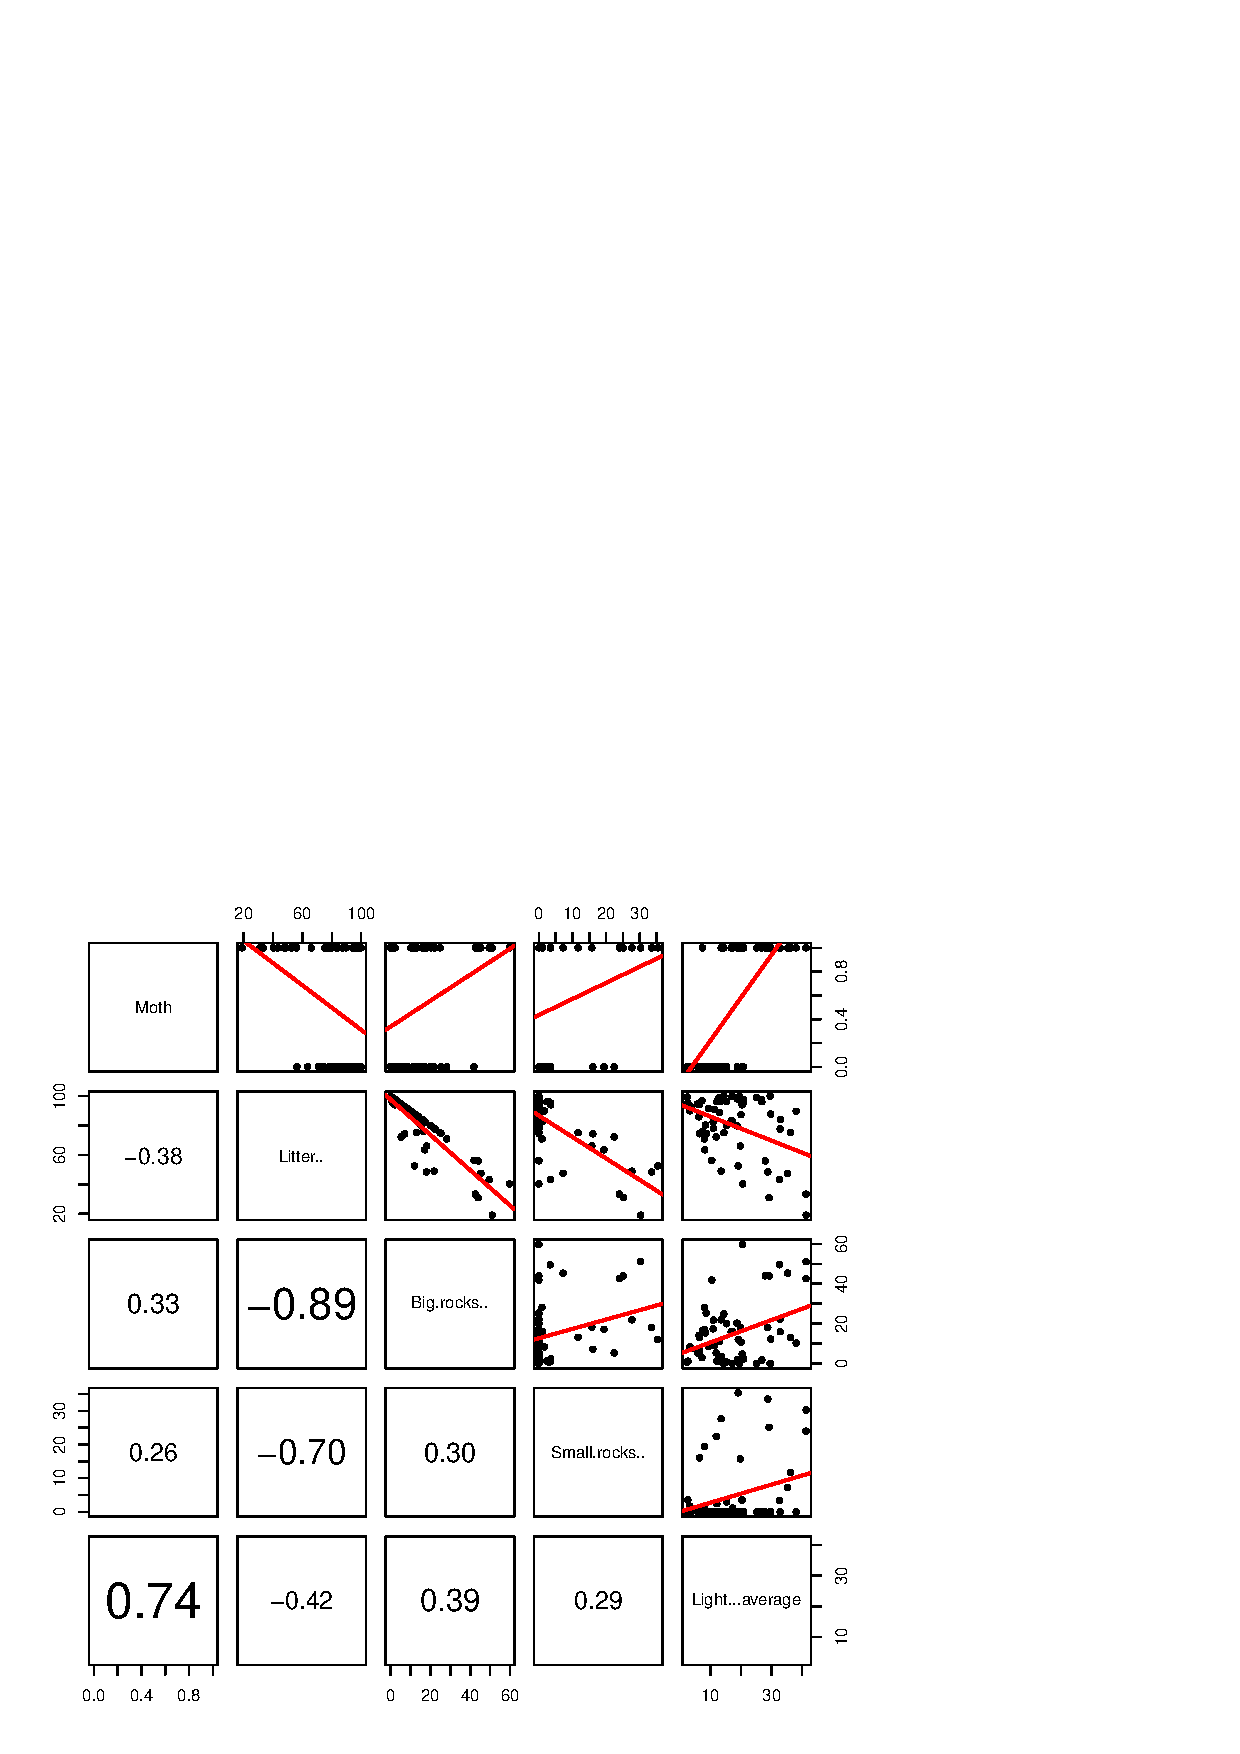
\includegraphics{SCRL_tex-014}

\subsection{Moth Resistance Factors Affecting Abundance, Richness and Diversity}

\subsubsection{Abundance}
\begin{Schunk}
\begin{Sinput}
> par(mfrow = c(1, 3))
> hist(residuals(lm(a ~ Litter.. + Big.rocks.. + Small.rocks.. + 
+     Light...average + Moth)), main = "untransformed")
> log.a = log(a + 1e-07)
> hist(residuals(lm(log.a ~ Litter.. + Big.rocks.. + Small.rocks.. + 
+     Light...average + Moth)), main = "log transformed")
> sqrt.a = sqrt(a)
> hist(residuals(lm(sqrt.a ~ Litter.. + Big.rocks.. + Small.rocks.. + 
+     Light...average + Moth)), main = "sqrt transformed")
> summary(lm(a ~ Litter.. + Big.rocks.. + Small.rocks.. + 
+     Light...average + Moth))
\end{Sinput}
\begin{Soutput}
Call:
lm(formula = a ~ Litter.. + Big.rocks.. + Small.rocks.. + Light...average + 
    Moth)

Residuals:
    Min      1Q  Median      3Q     Max 
-3.1072 -0.8651 -0.3544  0.2685  7.2474 

Coefficients:
                Estimate Std. Error t value Pr(>|t|)    
(Intercept)     85.24680   21.82436   3.906 0.000263 ***
Litter..        -0.85572    0.22000  -3.890 0.000277 ***
Big.rocks..     -0.77126    0.22359  -3.449 0.001097 ** 
Small.rocks..   -0.87067    0.21868  -3.981 0.000206 ***
Light...average  0.04653    0.04168   1.116 0.269228    
Moth            -0.25567    0.83501  -0.306 0.760638    
---
Signif. codes:  0 ‘***’ 0.001 ‘**’ 0.01 ‘*’ 0.05 ‘.’ 0.1 ‘ ’ 1 

Residual standard error: 2.039 on 54 degrees of freedom
Multiple R-squared: 0.4695,	Adjusted R-squared: 0.4204 
F-statistic: 9.558 on 5 and 54 DF,  p-value: 1.422e-06 
\end{Soutput}
\begin{Sinput}
> summary(lm(sqrt.a ~ Litter.. + Big.rocks.. + Small.rocks.. + 
+     Light...average + Moth))
\end{Sinput}
\begin{Soutput}
Call:
lm(formula = sqrt.a ~ Litter.. + Big.rocks.. + Small.rocks.. + 
    Light...average + Moth)

Residuals:
     Min       1Q   Median       3Q      Max 
-1.08070 -0.38246 -0.07297  0.27107  1.74901 

Coefficients:
                Estimate Std. Error t value Pr(>|t|)    
(Intercept)     25.77513    6.98099   3.692 0.000519 ***
Litter..        -0.25605    0.07037  -3.639 0.000614 ***
Big.rocks..     -0.22174    0.07152  -3.100 0.003069 ** 
Small.rocks..   -0.26658    0.06995  -3.811 0.000357 ***
Light...average  0.02302    0.01333   1.727 0.089900 .  
Moth            -0.18254    0.26710  -0.683 0.497265    
---
Signif. codes:  0 ‘***’ 0.001 ‘**’ 0.01 ‘*’ 0.05 ‘.’ 0.1 ‘ ’ 1 

Residual standard error: 0.6522 on 54 degrees of freedom
Multiple R-squared: 0.5372,	Adjusted R-squared: 0.4944 
F-statistic: 12.54 on 5 and 54 DF,  p-value: 4.292e-08 
\end{Soutput}
\end{Schunk}
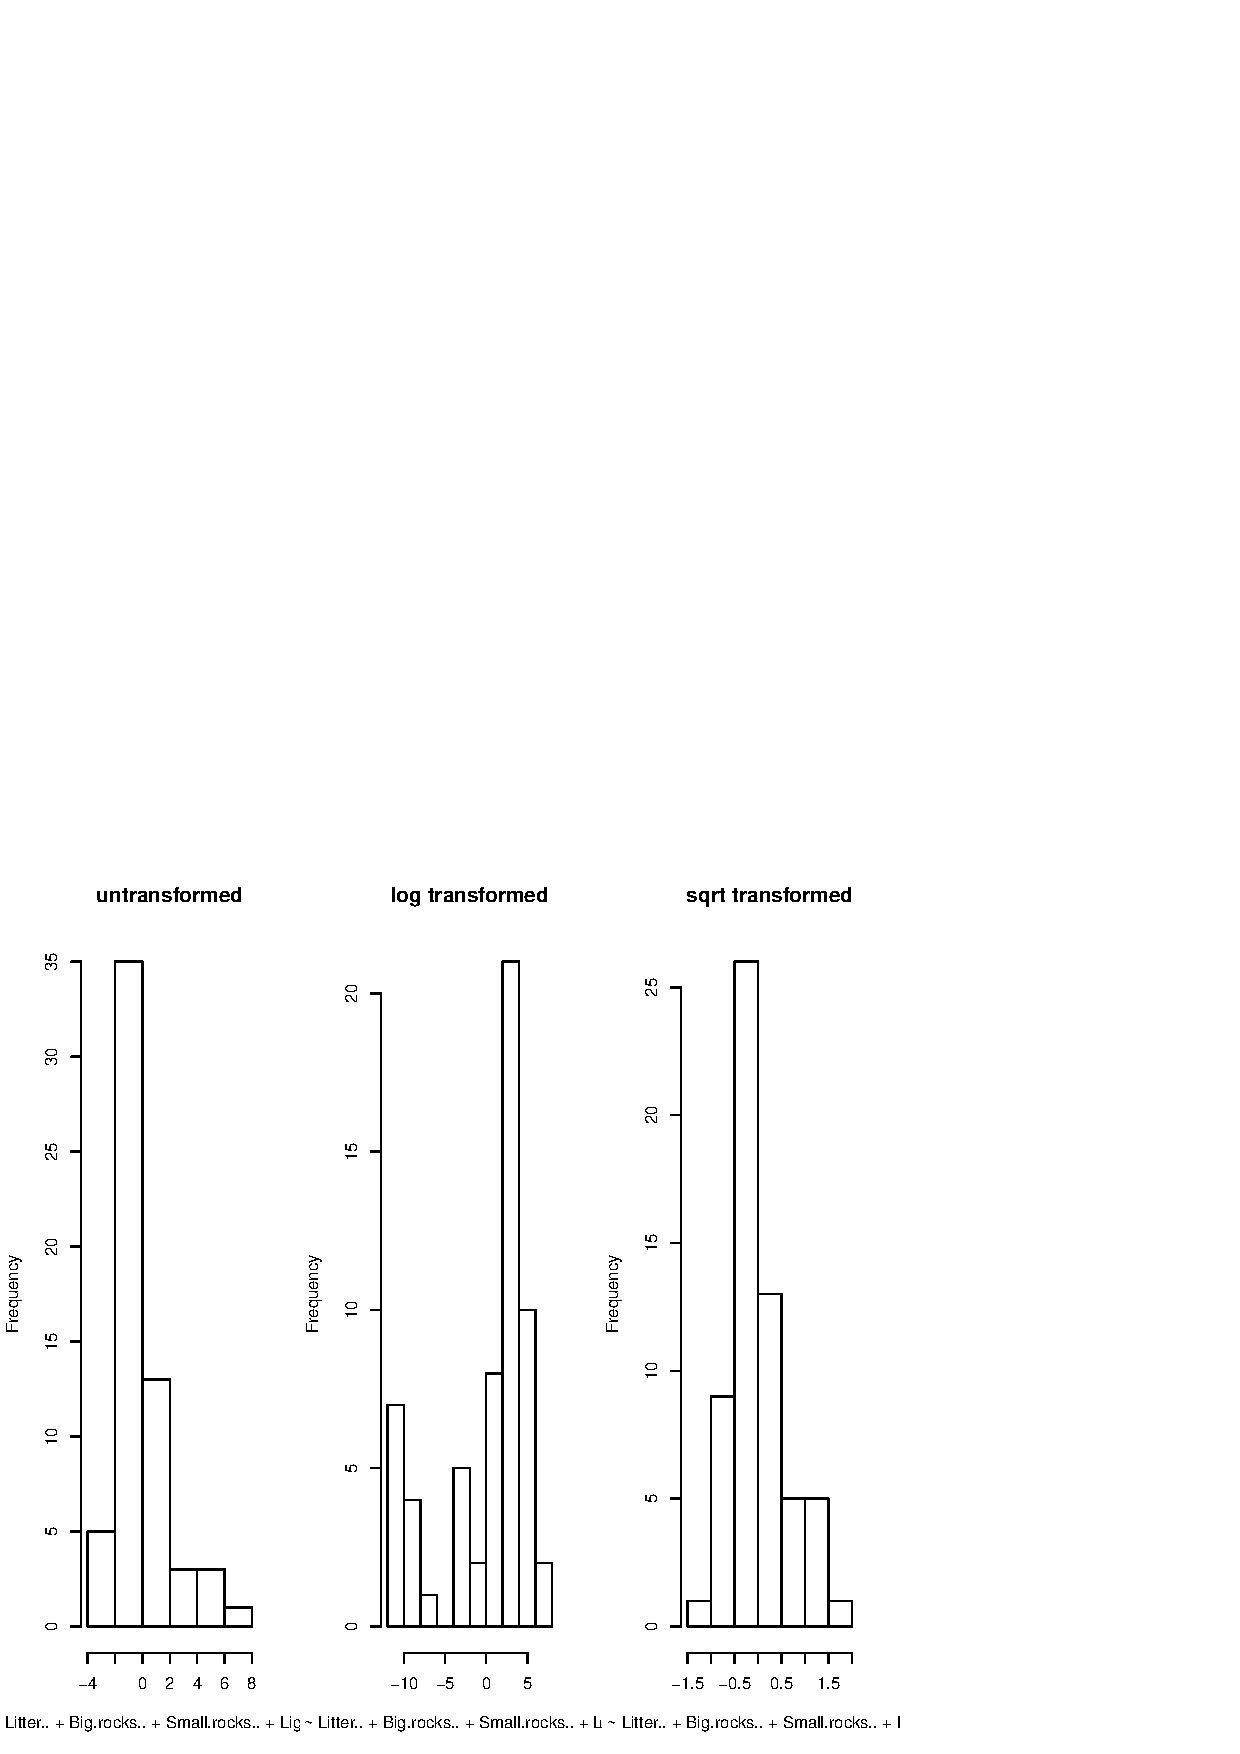
\includegraphics{SCRL_tex-015}

\subsubsection{Richness}
\begin{Schunk}
\begin{Sinput}
> par(mfrow = c(1, 3))
> hist(residuals(lm(r ~ Litter.. + Big.rocks.. + Small.rocks.. + 
+     Light...average + Moth)), main = "untransformed")
> hist(residuals(lm(sqrt(r) ~ Litter.. + Big.rocks.. + 
+     Small.rocks.. + Light...average + Moth)), main = "sqrt transformed")
> hist(residuals(lm(r^2 ~ Litter.. + Big.rocks.. + Small.rocks.. + 
+     Light...average + Moth)), main = "square transformed")
> summary(lm(r ~ Litter.. + Big.rocks.. + Small.rocks.. + 
+     Light...average + Moth))
\end{Sinput}
\begin{Soutput}
Call:
lm(formula = r ~ Litter.. + Big.rocks.. + Small.rocks.. + Light...average + 
    Moth)

Residuals:
    Min      1Q  Median      3Q     Max 
-4.4856 -1.8706 -0.3768  1.7516  5.6450 

Coefficients:
                Estimate Std. Error t value Pr(>|t|)  
(Intercept)     57.22541   26.76674   2.138   0.0371 *
Litter..        -0.56141    0.26982  -2.081   0.0422 *
Big.rocks..     -0.42130    0.27422  -1.536   0.1303  
Small.rocks..   -0.61029    0.26820  -2.275   0.0269 *
Light...average  0.09404    0.05112   1.840   0.0713 .
Moth            -0.23426    1.02410  -0.229   0.8199  
---
Signif. codes:  0 ‘***’ 0.001 ‘**’ 0.01 ‘*’ 0.05 ‘.’ 0.1 ‘ ’ 1 

Residual standard error: 2.501 on 54 degrees of freedom
Multiple R-squared: 0.5392,	Adjusted R-squared: 0.4965 
F-statistic: 12.64 on 5 and 54 DF,  p-value: 3.856e-08 
\end{Soutput}
\begin{Sinput}
> summary(lm(r^2 ~ Litter.. + Big.rocks.. + Small.rocks.. + 
+     Light...average + Moth))
\end{Sinput}
\begin{Soutput}
Call:
lm(formula = r^2 ~ Litter.. + Big.rocks.. + Small.rocks.. + Light...average + 
    Moth)

Residuals:
   Min     1Q Median     3Q    Max 
-33.42 -16.67  -5.87  11.72  78.40 

Coefficients:
                Estimate Std. Error t value Pr(>|t|)  
(Intercept)     579.1453   263.4597   2.198   0.0322 *
Litter..         -5.8314     2.6558  -2.196   0.0324 *
Big.rocks..      -4.4782     2.6991  -1.659   0.1029  
Small.rocks..    -6.2763     2.6399  -2.378   0.0210 *
Light...average   1.0309     0.5031   2.049   0.0453 *
Moth             -0.5560    10.0801  -0.055   0.9562  
---
Signif. codes:  0 ‘***’ 0.001 ‘**’ 0.01 ‘*’ 0.05 ‘.’ 0.1 ‘ ’ 1 

Residual standard error: 24.61 on 54 degrees of freedom
Multiple R-squared: 0.5571,	Adjusted R-squared: 0.5161 
F-statistic: 13.58 on 5 and 54 DF,  p-value: 1.384e-08 
\end{Soutput}
\end{Schunk}
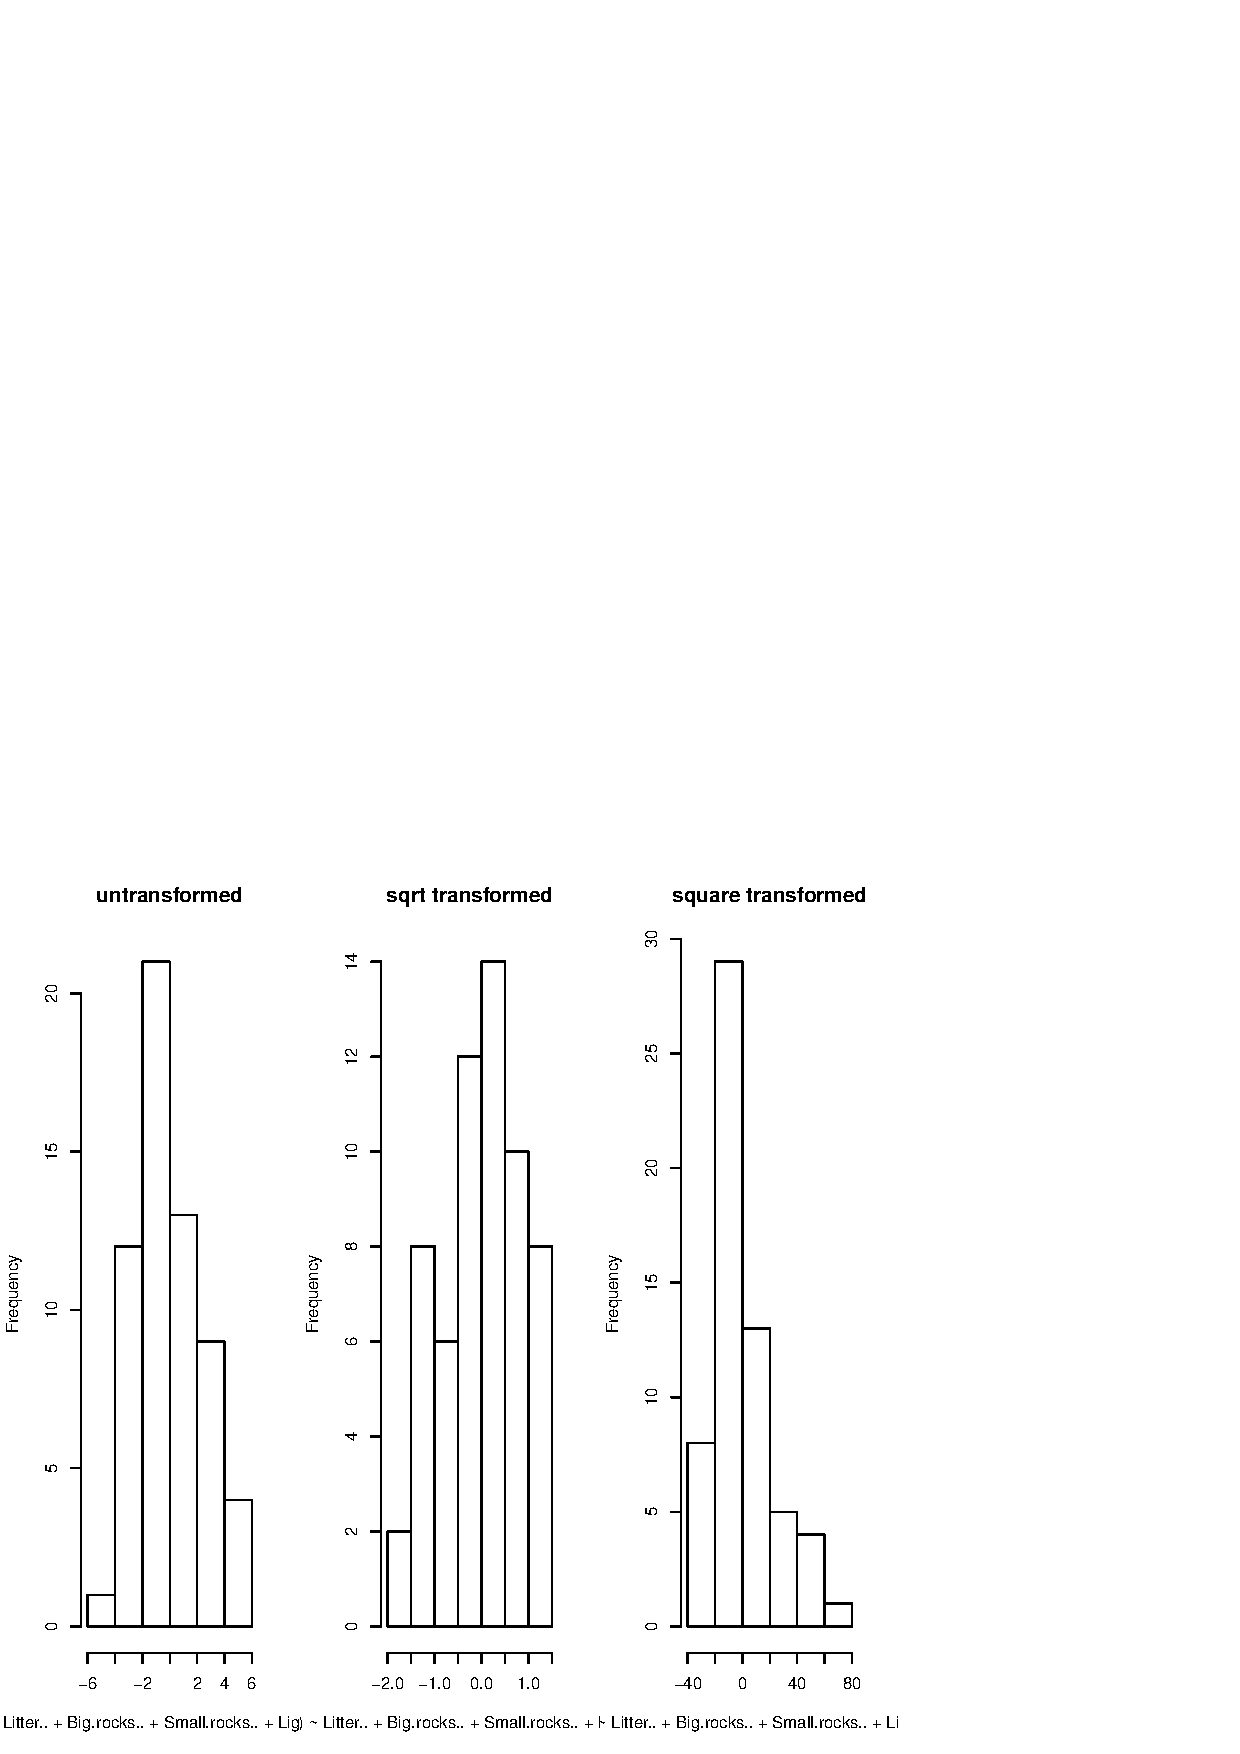
\includegraphics{SCRL_tex-016}

\subsubsection{Diversity}
\begin{Schunk}
\begin{Sinput}
> par(mfrow = c(2, 2))
> hist(residuals(lm(h ~ Litter.. + Big.rocks.. + Small.rocks.. + 
+     Light...average + Moth)), main = "untransformed")
> hist(residuals(lm(h^2 ~ Litter.. + Big.rocks.. + Small.rocks.. + 
+     Light...average + Moth)), main = "square transformed")
> hist(residuals(lm(sqrt(h) ~ Litter.. + Big.rocks.. + 
+     Small.rocks.. + Light...average + Moth)), main = "sqrt transformed")
> hist(residuals(lm(log(h + 1e-07) ~ Litter.. + Big.rocks.. + 
+     Small.rocks.. + Light...average + Moth)), main = "log transformed")
> summary(lm(h ~ Litter.. + Big.rocks.. + Small.rocks.. + 
+     Light...average + Moth))
\end{Sinput}
\begin{Soutput}
Call:
lm(formula = h ~ Litter.. + Big.rocks.. + Small.rocks.. + Light...average + 
    Moth)

Residuals:
     Min       1Q   Median       3Q      Max 
-0.94610 -0.48766 -0.06364  0.58525  0.99877 

Coefficients:
                 Estimate Std. Error t value Pr(>|t|)
(Intercept)      2.176658   5.855802   0.372    0.712
Litter..        -0.018851   0.059029  -0.319    0.751
Big.rocks..      0.007832   0.059992   0.131    0.897
Small.rocks..   -0.025606   0.058675  -0.436    0.664
Light...average  0.015461   0.011183   1.383    0.173
Moth            -0.029532   0.224045  -0.132    0.896

Residual standard error: 0.5471 on 54 degrees of freedom
Multiple R-squared: 0.437,	Adjusted R-squared: 0.3849 
F-statistic: 8.384 on 5 and 54 DF,  p-value: 6.401e-06 
\end{Soutput}
\begin{Sinput}
> summary(lm(h^2 ~ Litter.. + Big.rocks.. + Small.rocks.. + 
+     Light...average + Moth))
\end{Sinput}
\begin{Soutput}
Call:
lm(formula = h^2 ~ Litter.. + Big.rocks.. + Small.rocks.. + Light...average + 
    Moth)

Residuals:
    Min      1Q  Median      3Q     Max 
-1.5414 -0.6235 -0.2444  0.7020  1.7744 

Coefficients:
                  Estimate Std. Error t value Pr(>|t|)
(Intercept)      0.1782364  9.8765336   0.018    0.986
Litter..        -0.0003917  0.0995594  -0.004    0.997
Big.rocks..      0.0473428  0.1011843   0.468    0.642
Small.rocks..   -0.0106344  0.0989632  -0.107    0.915
Light...average  0.0310721  0.0188615   1.647    0.105
Moth            -0.0350014  0.3778796  -0.093    0.927

Residual standard error: 0.9227 on 54 degrees of freedom
Multiple R-squared: 0.4827,	Adjusted R-squared: 0.4348 
F-statistic: 10.08 on 5 and 54 DF,  p-value: 7.49e-07 
\end{Soutput}
\end{Schunk}
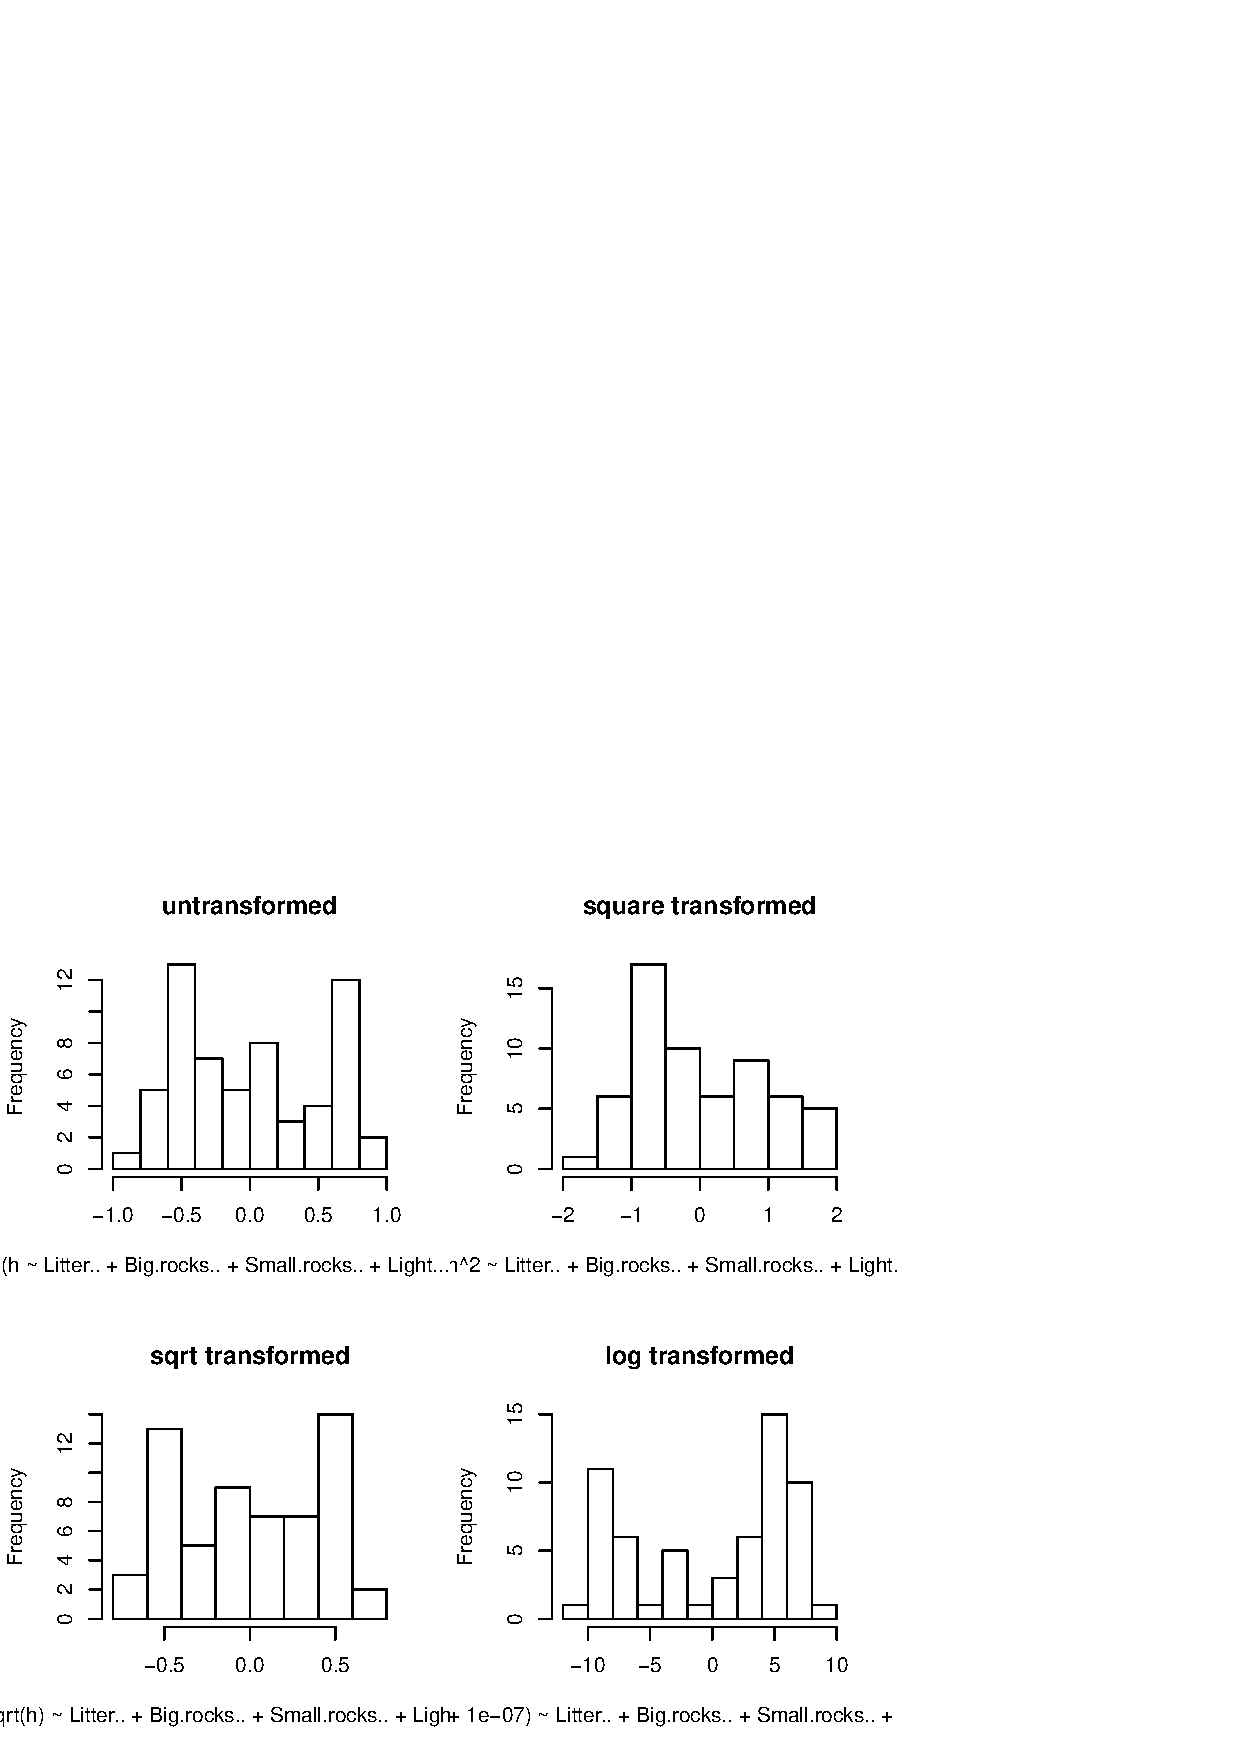
\includegraphics{SCRL_tex-017}

\subsection{Factors Resistance Factors Affecting the Community}
\begin{Schunk}
\begin{Sinput}
> adonis(d ~ Litter.. + Big.rocks.. + Small.rocks.. + Light...average + 
+     Moth, permutations = 9999)
\end{Sinput}
\begin{Soutput}
Call:
adonis(formula = d ~ Litter.. + Big.rocks.. + Small.rocks.. +      Light...average + Moth, permutations = 9999) 

                      Df SumsOfSqs  MeanSqs  F.Model     R2 Pr(>F)
Litter..         1.00000   2.02064  2.02064  6.85110 0.1002 0.0002
Big.rocks..      1.00000   1.02549  1.02549  3.47698 0.0509 0.0045
Small.rocks..    1.00000   0.44991  0.44991  1.52546 0.0223 0.1373
Light...average  1.00000   0.42702  0.42702  1.44784 0.0212 0.1772
Moth             1.00000   0.30983  0.30983  1.05049 0.0154 0.3618
Residuals       54.00000  15.92658  0.29494          0.7900       
Total           59.00000  20.15947                   1.0000       
                   
Litter..        ***
Big.rocks..     ** 
Small.rocks..      
Light...average    
Moth               
Residuals          
Total              
---
Signif. codes:  0 ‘***’ 0.001 ‘**’ 0.01 ‘*’ 0.05 ‘.’ 0.1 ‘ ’ 1 
\end{Soutput}
\end{Schunk}


\subsection{Structural Equation Modeling}

\subsection{Notes on the SEMs}

\begin{description}
\item[ ] SEM allows us to account for and isolate the covariances in multiple correlated variables. 
\item This is not the same as conducting an experiment, but it gives us more accurate information than multiple regressions because we can assess both the direct and \textit{indirect}, sometimes termed informally as interactive, effects of variables.
\item Numbers above paths in the path diagrams are standardized path coefficient, which can be thought of as the amount of change one variable due to another variable in standard deviations. 
\item The numbers next to the top right corner of variables that are endogenous (i.e., there are arrows pointing into them) are squared multiple correlations, which can be treated as multiple $r^2$ (i.e., the total variance explained in that variable by all the variables pointing into it).
\item Things to look for and remember:
\begin{enumerate}
\item SEM works by testing \textit{a priori} models against the data.
\item In the notes for the models, a small $\chi^2$ and a large p-value indicate good model fit, because it shows that the model predicted covariances are statistically similar to the raw covariances.
\item There are two main pathways in each model, one is a path through Average Light (variable name = \texttt{Light...average}) and the other is a more complex path through percent litter (variable name = \texttt{Litter..}) and percent rocks > 3cm (variable name = \texttt{Big.rocks..}).
\item In addition to whole model fit, we also need to look at the significance of each path, which can be done by looking at the regression weights output (NOTE: the asterisks indicate that a variable is significant below 0.001).
\end{enumerate}

\item I built the \textit{a priori} models based on what we have discussed about the system and the multiple regressions. 

\item I have also presented the model modification output, which would indicate variables in the model that need to be changed; however, we had not variables recommended for change, another suggestion of the validity of our models. 

\item Here I use \texttt{resistance}, such that \texttt{resistance} increases from 0 = susceptible to 1 = resistant. This makes more intuitive sense than \texttt{Moth}, but is numerically equivalent.

\end{description}


\subsubsection{Abundance}

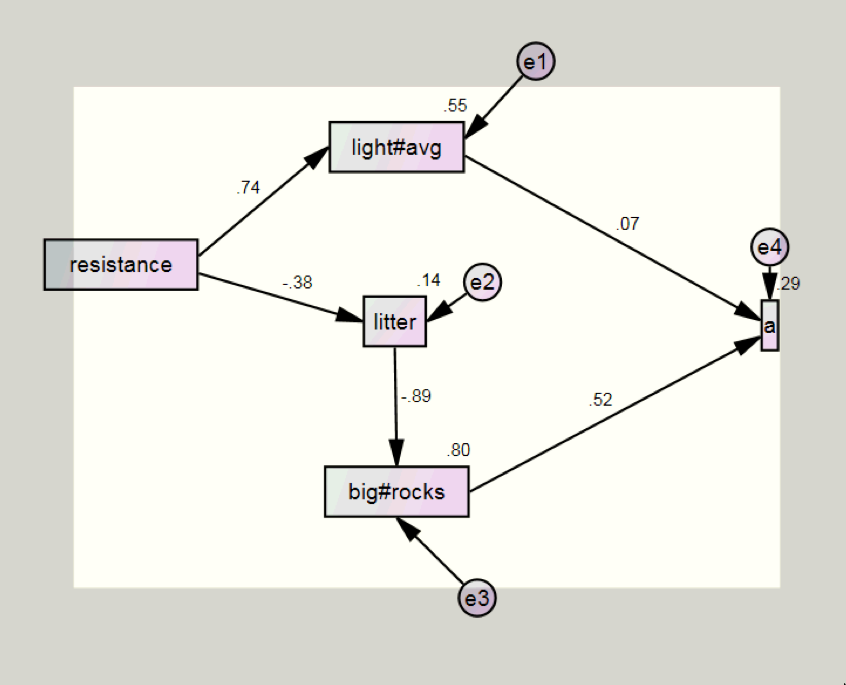
\includegraphics[]{A_SEMpathdia.png}

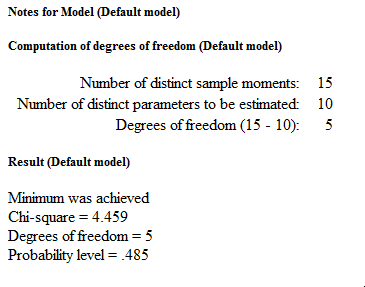
\includegraphics[]{A_SEMnotes.png}

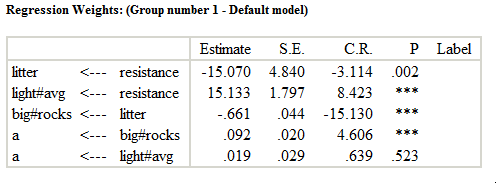
\includegraphics[]{A_SEMreg.png}

\subsubsection{Richness}

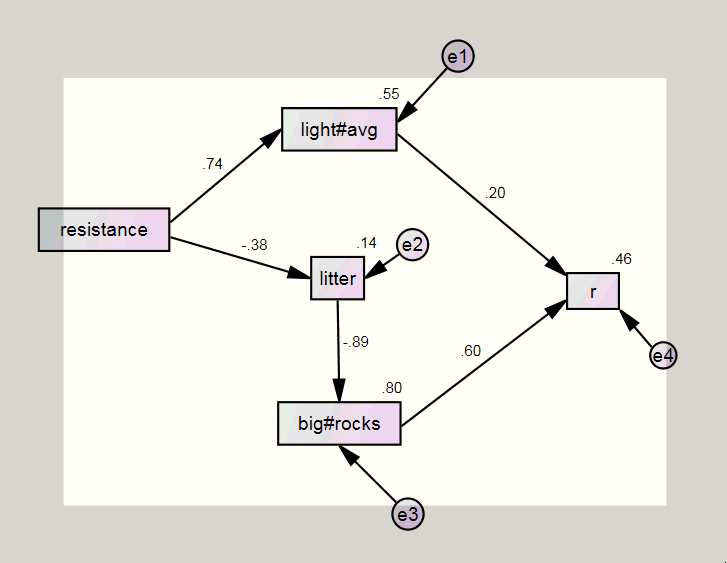
\includegraphics[]{R_SEMpathdia.png}

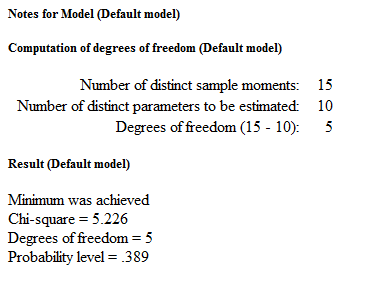
\includegraphics[]{R_SEMnotes.png}

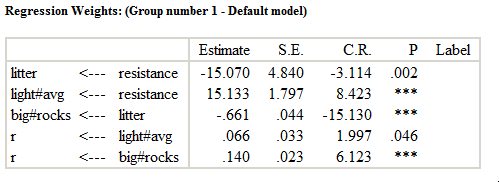
\includegraphics[]{R_SEMreg.png}


\subsubsection{Diversity}

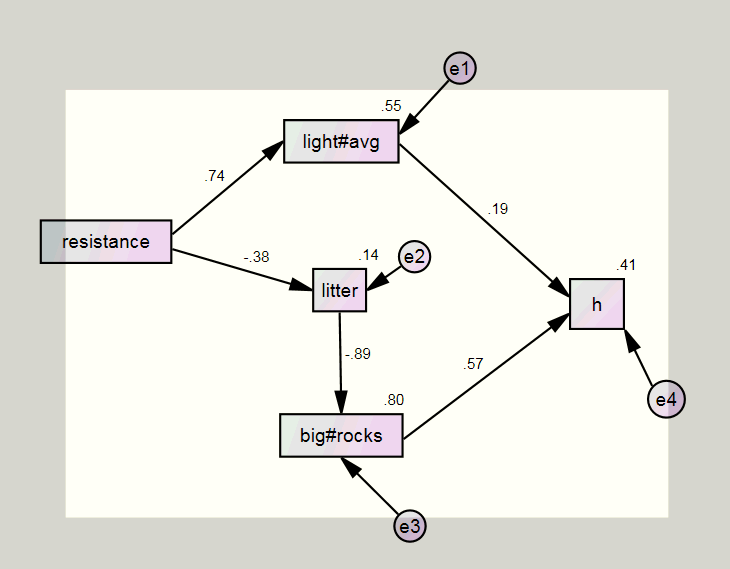
\includegraphics[]{H_SEMpathdia.png}

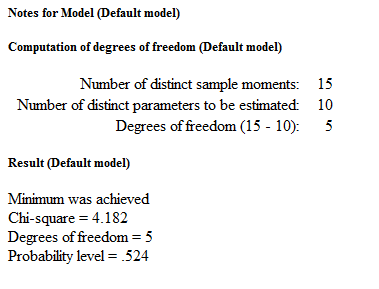
\includegraphics[]{H_SEMnotes.png}

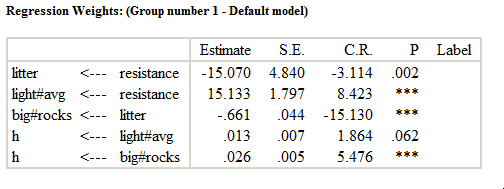
\includegraphics[]{H_SEMreg.png}

\subsubsection{Community Composition}

\textbf{NOTE:} I need to confer with other folks (Matt Bowker, Daniel Laughlin and Jamie Lamit) on the best way to approach our SEM based analysis of community composition.


\section{Conclusion}

\begin{enumerate}
\item Based on univariate and multivariate statistical analyses of the effect of moth susceptibility, we can conclude that moth susceptibility has a statistically significant effect on rock lichen epiphyte abundance, richness, diversity and community composition with multiple species changing in response (see the indicator species analyses).
\item The analyses of the predictor variables and moth susceptibility suggested that there were several key factors related to moth susceptibility: percent rocks > 3cm, percent litter cover and average incident light.
\item SEM models indicate that there the effect of moth resistance on rock lichen/moss abundance, species richness and diversity is primarily due to an indirect effect where resistance has a negative effect on the abundance of litter, which also has a negative effect on the abundance of percent large rocks. Thus, because there is a positive relationship between percent large rocks and abundance, species richness and diversity, the net, indirect, effect of resistance on rock lichen/moss communities is positive.
\end{enumerate}

Thus, we can conclude that evolutionary shifts in \textit{Pinus edulis} moth susceptibility could have significant community level consequences for sub-canopy rock lichen/moss communities. 

\end{document}
